% ============================================================================
%  From a witness of quantumness to a bosonic code and back to the hardware:
%  the spider state, rotation-symmetric codes, and a drive-tuned CROT gate
%
%  Written for Physical Review A (REVTeX 4.2).  If REVTeX is not installed the
%  file falls back to the standard article class so that it still compiles;
%  the content is identical, only the layout differs.
%
%  Build:  pdflatex main && bibtex main && pdflatex main && pdflatex main
% ============================================================================
\IfFileExists{revtex4-2.cls}{%
  \documentclass[aps,pra,reprint,superscriptaddress,amsmath,amssymb,nofootinbib]{revtex4-2}
  \newcommand{\revtexfallback}{0}%
}{%
  \documentclass[10pt,twocolumn]{article}
  \usepackage[a4paper,margin=1.8cm]{geometry}
  \usepackage{amsmath,amssymb}
  \usepackage[numbers,sort&compress]{natbib}
  \newcommand{\revtexfallback}{1}%
}
\ifnum\revtexfallback=1
  % minimal stand-ins for the REVTeX front-matter and float commands
  \newcommand{\affiliation}[1]{\\[-0.2em]{\small\itshape #1}}
  \newcommand{\preprint}[1]{}
  \newenvironment{ruledtabular}{\begin{center}}{\end{center}}
  \newenvironment{acknowledgments}{\section*{Acknowledgments}}{}
\fi
\usepackage{graphicx}
\usepackage{bm}
\usepackage{hyperref}
\graphicspath{{figures/}}

\newcommand{\pos}{\mathrm{pos}}
\newcommand{\ket}[1]{|#1\rangle}
\newcommand{\bra}[1]{\langle#1|}
\newcommand{\braket}[2]{\langle#1|#2\rangle}
\newcommand{\n}{\hat n}
\newcommand{\Pc}{\mathbf{P}^{c}}
\newcommand{\Pq}{\mathbf{P}^{\infty}}

\begin{document}

\title{From a witness of quantumness to a bosonic code and back to the hardware:\\
the spider state, rotation-symmetric codes, and a drive-tuned CROT gate}

\ifnum\revtexfallback=1
\author{Tien D. Nguyen\affiliation{Centre for Quantum Technologies, National University of Singapore, 117543 Singapore}\affiliation{Faculty of Physics, Hanoi University of Science, VNU Hanoi, 120401 Vietnam}}
\else
\author{Tien D. Nguyen}
\affiliation{Centre for Quantum Technologies, National University of Singapore, 117543 Singapore}
\affiliation{Faculty of Physics, Hanoi University of Science, VNU Hanoi, 120401 Vietnam}
\fi

\ifnum\revtexfallback=1
  \date{\today}
  \twocolumn[
  \begin{@twocolumnfalse}
  \maketitle
  \begin{abstract}
  Rotation-symmetric bosonic codes encode a qubit in the Fock states $\ket{mK}$ of a single oscillator. We follow a primitive that was found for an unrelated reason: the \textsc{spider} state, which maximally violates the classical bound of the precession protocol of Zaw \emph{et al.} [Phys.\ Rev.\ A \textbf{106}, 032222 (2022)] and happens to have exactly the required $K$-fold rotation symmetry. We show that the score operator of the protocol is block diagonal in the rotation-symmetry sectors, so that the spider state defines an order-$K$ code whose preparation can be certified device-independently from sign measurements alone, with a spectral-gap fidelity witness. The code, however, is not error-correcting: its codewords carry mean photon numbers in a fixed ratio of three, the Knill--Laflamme non-deformation condition fails by an amount of order the photon number, no finite reweighting of the coefficients can repair it without abandoning the maximal violation that defines the state, and the exact state has infinite mean energy. Since the obstacle to rotation-code error correction is then not the primitive but the gadgets, we turn to the controlled-rotation gate $e^{i\varphi\n\otimes\n}$ that every rotation code needs and engineer it from the drive-tuned cross-Kerr interaction between two superconducting cavities sharing a transmon. An untargeted drive enhances the cross-Kerr four-fold and yields a gate time of tens of microseconds, but produces self-Kerr of comparable size; a 99\% gate tolerates a residual self-Kerr below one percent of the cross-Kerr. We then reproduce, with the same dressed-ladder numerics, the single-tone drive-enhanced scheme that completed the project [Qin \emph{et al.}, arXiv:2609.07076]: a drive placed next to the two-cavity conversion resonance raises the cross-Kerr on-off ratio above fifty while the self-Kerrs stay small, and a driven side transmon---already present in recovered four-mode simulations---cancels the residual, leaving the data rail of the CROT gate exact in the diagonal model.

  \end{abstract}
  \vspace{1em}
  \end{@twocolumnfalse}
  ]
\else
  \date{\today}
  \begin{abstract}
  Rotation-symmetric bosonic codes encode a qubit in the Fock states $\ket{mK}$ of a single oscillator. We follow a primitive that was found for an unrelated reason: the \textsc{spider} state, which maximally violates the classical bound of the precession protocol of Zaw \emph{et al.} [Phys.\ Rev.\ A \textbf{106}, 032222 (2022)] and happens to have exactly the required $K$-fold rotation symmetry. We show that the score operator of the protocol is block diagonal in the rotation-symmetry sectors, so that the spider state defines an order-$K$ code whose preparation can be certified device-independently from sign measurements alone, with a spectral-gap fidelity witness. The code, however, is not error-correcting: its codewords carry mean photon numbers in a fixed ratio of three, the Knill--Laflamme non-deformation condition fails by an amount of order the photon number, no finite reweighting of the coefficients can repair it without abandoning the maximal violation that defines the state, and the exact state has infinite mean energy. Since the obstacle to rotation-code error correction is then not the primitive but the gadgets, we turn to the controlled-rotation gate $e^{i\varphi\n\otimes\n}$ that every rotation code needs and engineer it from the drive-tuned cross-Kerr interaction between two superconducting cavities sharing a transmon. An untargeted drive enhances the cross-Kerr four-fold and yields a gate time of tens of microseconds, but produces self-Kerr of comparable size; a 99\% gate tolerates a residual self-Kerr below one percent of the cross-Kerr. We then reproduce, with the same dressed-ladder numerics, the single-tone drive-enhanced scheme that completed the project [Qin \emph{et al.}, arXiv:2609.07076]: a drive placed next to the two-cavity conversion resonance raises the cross-Kerr on-off ratio above fifty while the self-Kerrs stay small, and a driven side transmon---already present in recovered four-mode simulations---cancels the residual, leaving the data rail of the CROT gate exact in the diagonal model.

  \end{abstract}
  \maketitle
\fi

% ----------------------------------------------------------------------------
\section{Introduction}
% ----------------------------------------------------------------------------
Bosonic quantum error correction (QEC) replaces the many physical qubits of a
conventional code by the many levels of a single oscillator
\cite{chuang1997,gkp2001,joshi2021}. The redundancy is free, the dominant error
(photon loss) is simple, and the hardware---three-dimensional superconducting
cavities read out by a transmon ancilla---is mature enough that a cat code
\cite{ofek2016} and more recently a GKP code \cite{sivak2023} have been
operated beyond the break-even point. Among single-mode codes, the family
defined by a discrete rotation symmetry in phase space, the
\emph{rotation-symmetric bosonic} (RSB) codes of \cite{grimsmo2020}, is particularly attractive: it contains the cat
\cite{mirrahimi2014} and binomial \cite{michael2016} codes, its distance is set
by a single integer $K$, and it comes with a complete gate set and a
teleportation-based error-correction gadget built from two primitives, a
controlled-rotation gate $\mathrm{CROT}(\varphi)=e^{i\varphi\n\otimes\n}$ and a
phase measurement.

The physics of RSB codes is, to a large extent, the physics of the
\emph{primitive state} from which the codewords are built. A coherent state
gives a cat code, a binomial amplitude profile gives a binomial code, a phase
state gives the number-phase code. It is therefore natural to ask whether other
states with $K$-fold rotation symmetry---states found for entirely different
reasons---make interesting codes. The present work follows one such candidate
from its discovery to its verdict, and then to the hardware question that the
verdict leaves standing.

The candidate comes from the foundations of quantum mechanics. Tsirelson
\cite{tsirelson2006} and, in a general form Zaw \textit{et al.} \cite{zaw2022} showed that a harmonic oscillator in uniform precession obeys a
classical bound on the probability of finding its coordinate positive when
sampled at $K$ equally spaced times, and that this bound is violated by quantum
states. The state that violates it \emph{maximally} has support only on the
Fock states $\ket{mK}$, and its Wigner function has $K$ legs of negativity
emanating from the origin: the \textsc{spider} state. Because support on
$\ket{mK}$ is precisely the definition of a logical $\ket{+}$ of an order-$K$
RSB code, the spider state is a code in waiting, and a special one: it is the
only RSB primitive whose preparation can be certified from sign measurements
alone.

We ask three questions and answer each numerically with a small, open code
base. (i)~What are the properties of the spider state as a code primitive?
(ii)~Does the resulting spider code satisfy the Knill--Laflamme conditions
\cite{knill1997}? The answer is no, and we show why no finite repair of the
coefficients can change that. (iii)~Since the obstacle is not the primitive but
the gadgets, how good a CROT gate can be engineered between two cavities with
the drive-tuned cross-Kerr interaction of Zhang \emph{et al.}
\cite{zhang2022}? For the last question we present our generic exploration
and then the answer that the same group has since published, the single-tone
drive-enhanced CROT gate of Qin \emph{et al.} \cite{qin2026}, which we
reproduce with the same numerical tools. The paper is organised along these questions:
Sec.~\ref{sec:spider} introduces the precession protocol and the spider state,
Sec.~\ref{sec:code} builds the spider code, Sec.~\ref{sec:kl} delivers the
Knill--Laflamme verdict, and Sec.~\ref{sec:crot} turns to the cross-Kerr CROT
gate. Section~\ref{sec:outlook} concludes.

% ----------------------------------------------------------------------------
\section{The spider state}\label{sec:spider}
% ----------------------------------------------------------------------------
\subsection{Precession protocol and classical bound}
Consider an oscillator $H=\tfrac12(p^2+x^2)$ in units $\hbar=\omega=1$, so that
$x(t)$ precesses uniformly with period $T=2\pi$. In each run of the protocol
the state is prepared, one of $K$ times $t_k=kT/K$ ($k=0,\dots,K-1$) is drawn
at random, and the sign of $x$ is recorded. The score is the average
probability of a positive sign,
\begin{equation}
  P_K=\frac1K\sum_{k=0}^{K-1}\Pr[x(t_k)>0]. \label{eq:score}
\end{equation}
For \emph{any} classical state of the oscillator---any probability
distribution on phase space, however non-Gaussian---one has for odd $K$
\cite{tsirelson2006,zaw2022}
\begin{equation}
  P_K\le\Pc_K=\tfrac12\left(1+\tfrac1K\right),
\end{equation}
while for even $K$ the score is exactly $1/2$. The bound follows from the
observation that a classical trajectory visits the $K$ measurement angles in
turn, so at most $\lceil K/2\rceil$ of them can lie in the half-plane $x>0$.

Quantum mechanically $P_K=\bra\psi\hat Q_K\ket\psi$ with the score operator
\begin{equation}
  \hat Q_K=\frac1K\sum_{k=0}^{K-1}\hat U_k^\dagger\,\pos(\hat x)\,\hat U_k,
  \qquad \hat U_k=e^{-i\n t_k}, \label{eq:QK}
\end{equation}
where $\pos(\hat x)=\tfrac12(1+\mathrm{sgn}\,\hat x)$ projects on $x>0$. The
largest eigenvalue $\Pq_K$ of $\hat Q_K$ exceeds $\Pc_K$; its eigenvector is
the spider state $\ket{S_K}$.

\subsection{Rotation symmetry from the Kronecker comb}
The structure that connects the protocol to bosonic codes is elementary.
Since $\hat U_k\ket n=e^{-2\pi ink/K}\ket n$,
\begin{equation}
  (\hat Q_K)_{mn}=\pos_{mn}\,\frac1K\sum_{k=0}^{K-1}e^{2\pi i(m-n)k/K}
  =\pos_{mn}\,\delta_{m\equiv n\ (\mathrm{mod}\ K)} .
\end{equation}
The score operator is the projector $\pos(\hat x)$ with every matrix element
between Fock states of different residue modulo $K$ erased
(Fig.~\ref{fig:structure}). It is block diagonal in the residue classes, its
eigenvectors can be chosen inside one class, and the top eigenvector lives in
the class $n\equiv0$: it has support only on $\ket{mK}$ and is therefore an
eigenstate of the discrete rotation $\hat R_K=e^{2\pi i\n/K}$ with eigenvalue
$+1$. The matrix elements of $\pos(\hat x)$ themselves have the closed form
(Appendix~\ref{app:pos})
\begin{equation}
  \bra m\pos(\hat x)\ket n=\frac{\psi_n(0)\psi_m'(0)-\psi_m(0)\psi_n'(0)}{2(m-n)}
  \quad(m\neq n),
\end{equation}
with $\bra n\pos(\hat x)\ket n=\tfrac12$, so that truncations of $10^4$ Fock
states are diagonalised in seconds.

\begin{figure}[t]
  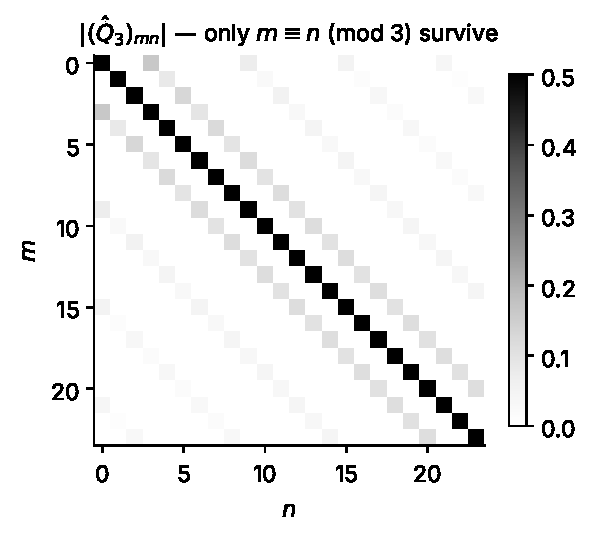
\includegraphics[width=0.7\columnwidth]{score_operator_structure_K3}
  \caption{\label{fig:structure}Modulus of the matrix elements of the score
  operator $\hat Q_3$ in the Fock basis. Only elements with $m\equiv n$
  (mod~3) survive the sum over measurement times, and within a residue class
  only $m-n$ odd multiples of 3 are non-zero (parity of $\pos(\hat x)$).}
\end{figure}

\subsection{Properties of the spider state}
Figure~\ref{fig:spider} summarises the numerics for $K=3$ (notebook 01 of the
repository). The Fock-grid coefficients $s_m=\braket{mK}{S_K}$ are real with
the sign pattern $(-1)^{\lceil m/2\rceil}$, $s_0=0.699$, $s_1=-0.515$,
$s_3=0.257$, in agreement with Ref.~\cite{zaw2022}. The score converges with
the truncation $n$ of the Fock grid (cutoff $Kn$) as a power law,
$P_3(n)=\Pq_3-0.040\,n^{-0.50}$, to
\begin{equation}
  \Pq_3=0.7094>\Pc_3=0.6667,
\end{equation}
and the $K$ measurement times contribute equally, as rotation symmetry
requires. For $K=5,7,9$ we find $\Pq_K=0.640,\,0.608,\,0.589$ against
$\Pc_K=0.600,\,0.571,\,0.556$, with spectral gaps $\epsilon=q_d-q_{d-1}$ of
$0.040$--$0.034$ to the next eigenvalue.

\begin{figure*}[t]
  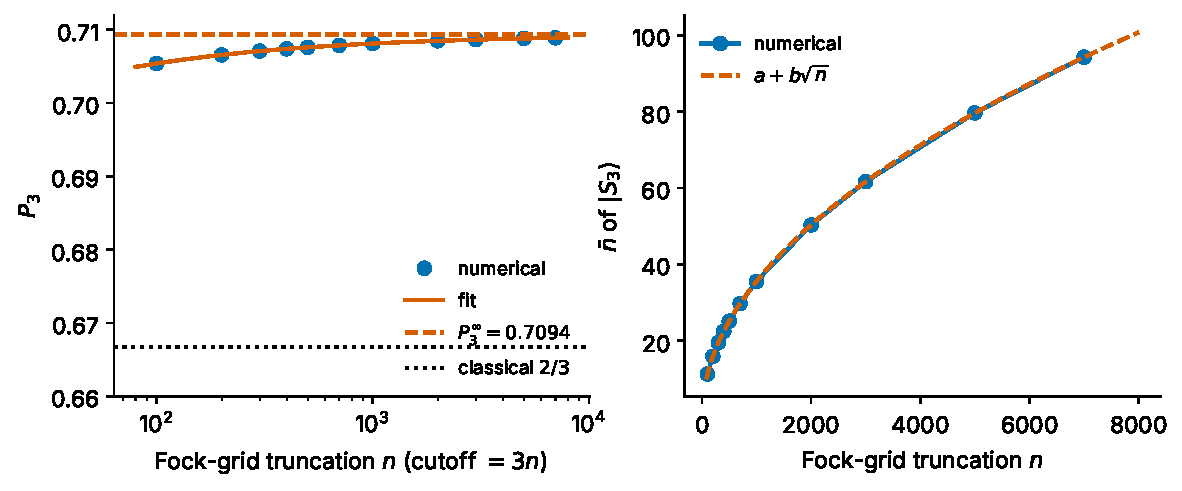
\includegraphics[width=0.62\textwidth]{spider_convergence_K3}\hfill
  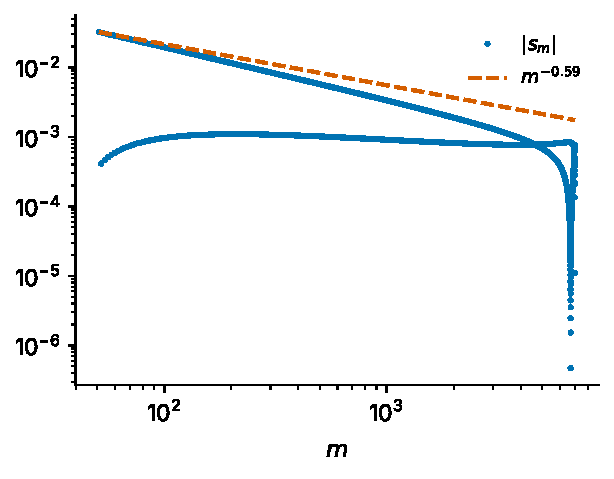
\includegraphics[width=0.36\textwidth]{spider_coefficient_tail_K3}
  \caption{\label{fig:spider}Left: score of the spider state $\ket{S_3}$
  against the Fock-grid truncation $n$ (dots), power-law fit (solid) and
  extrapolated $\Pq_3=0.7094$ (dashed); the classical bound is dotted.
  Middle: mean photon number of the truncated spider state, which grows as
  $\bar n\simeq1.13\sqrt n$ without saturating. Right: tail of the Fock-grid
  coefficients $|s_m|$ on a log-log scale; the decay is a power law with
  exponent between $-1/2$ and $-3/4$, i.e.\ $|s_m|^2$ decays slower than
  $m^{-3/2}$.}
\end{figure*}

The same figure shows the first warning sign. The mean photon number of the
truncated spider state grows as $\sqrt n$ and never saturates: the coefficient
tail decays so slowly that $\sum_m|s_m|^2$ converges but $\sum_m m|s_m|^2$ does
not. The exact spider state is normalisable but has \emph{infinite mean
energy}. Any physical preparation is a truncated approximation, and its
``size'' is a free parameter rather than a property of the code. The Wigner
functions (Fig.~\ref{fig:wigner}) show the $K$ legs of concentrated negativity
that give the state its name.

\begin{figure}[t]
  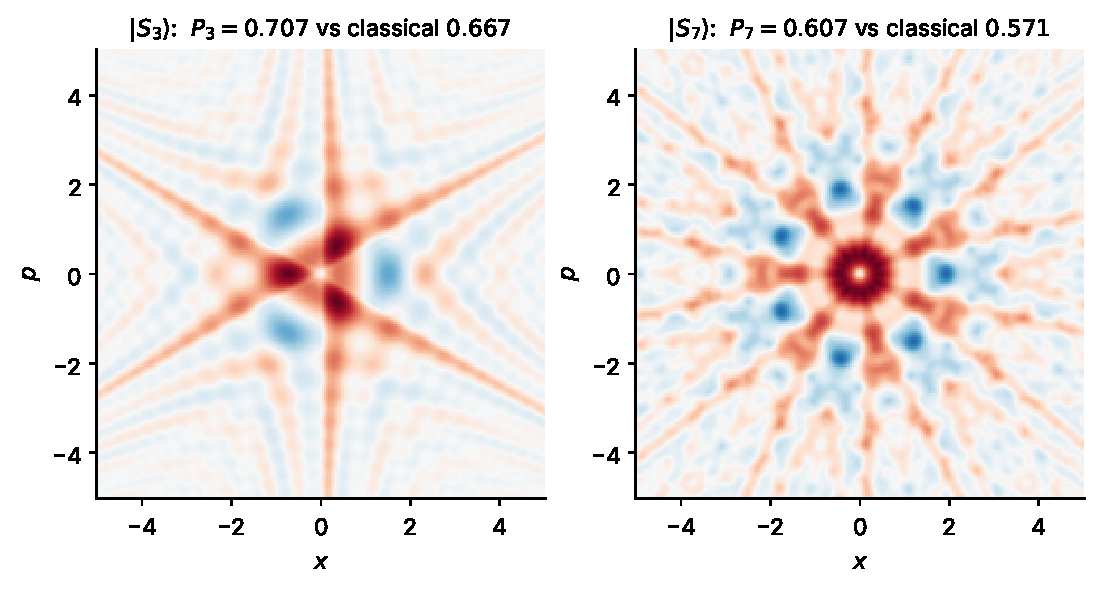
\includegraphics[width=\columnwidth]{spider_wigner_K3_K7}
  \caption{\label{fig:wigner}Wigner functions of the spider states for $K=3$
  and $K=7$ (truncated to 150 Fock states). Red is positive, blue negative.}
\end{figure}

% ----------------------------------------------------------------------------
\section{The spider code}\label{sec:code}
% ----------------------------------------------------------------------------
\subsection{Construction}
An order-$K$ RSB code \cite{grimsmo2020} is a two-dimensional subspace on which
$\hat Z_L=e^{i\pi\n/K}$ acts as the logical $Z$. The codewords are thus
supported on interleaved Fock grids,
\begin{equation}
  \ket{0_L}=\sum_m c_{2mK}\ket{2mK},\qquad
  \ket{1_L}=\sum_m c_{(2m+1)K}\ket{(2m+1)K},
\end{equation}
and the dual codewords $\ket{\pm_L}$ have support on every $\ket{mK}$. Any
normalised state on the full $K$-grid can be declared to be $\ket{+_L}$; the
Kronecker-comb projectors
$\hat\Pi^{\ell}_{2K}=\frac1{2K}\sum_{j=0}^{2K-1}(e^{-i\pi\ell/K}\hat Z_L)^j$
with $\ell=0,K$ then extract $\ket{0_L}$ and $\ket{1_L}$. We define the spider
code by $\ket{+_L}\equiv\ket{S_K}$. Numerically the codewords satisfy
$\hat Z_L\ket{0_L}=\ket{0_L}$, $\hat Z_L\ket{1_L}=-\ket{1_L}$ and
$\hat R_K\ket{\pm_L}=\ket{\pm_L}$ to machine precision
(Fig.~\ref{fig:codewords}).

\begin{figure*}[t]
  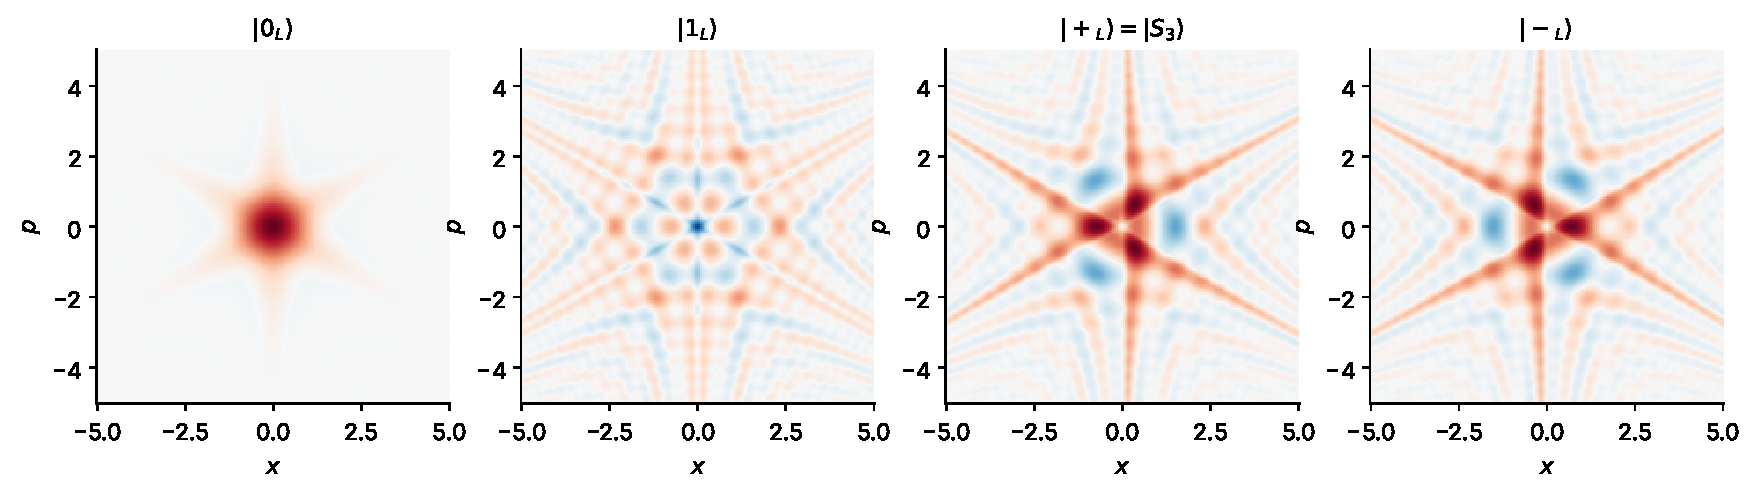
\includegraphics[width=0.95\textwidth]{spider_codewords_wigner_K3}
  \caption{\label{fig:codewords}Wigner functions of the spider-code codewords
  for $K=3$. $\ket{0_L}$ is 98\% vacuum; $\ket{1_L}$ has 53\% of its weight on
  $\ket3$; $\ket{-_L}$ is $\ket{+_L}=\ket{S_3}$ rotated by $\pi/3$.}
\end{figure*}

\subsection{Figures of merit}
The codewords are strikingly unequal. $\ket{0_L}$ is dominated by the vacuum
and $\ket{1_L}$ by $\ket 3$, and the mean photon numbers of the truncated
codewords are in the ratio $\bar n_1/\bar n_0\to3.00$ at every truncation
(Table~\ref{tab:nbar}), while both diverge. The embedded phase uncertainty
$\Delta_K(\theta)=|\langle e^{iK\theta}\rangle|^{-2}-1$, which controls how well
a code state serves as a phase reference in the error-correction gadget
\cite{grimsmo2020}, is $\Delta_3\simeq3.6$--$3.9$ for the spider state, an
order of magnitude larger than for cat, binomial or Pegg--Barnett primitives of
the same $\bar n$ (Fig.~\ref{fig:epu}): the energy in the long Fock tail does
nothing for the phase resolution.

\begin{table}[b]
\caption{\label{tab:nbar}Mean photon numbers of the spider codewords for
$K=3$ as a function of the Fock-grid truncation $n$ (cutoff $3n$).}
\begin{ruledtabular}
\begin{tabular}{rrrrr}
 $n$ & $\bar n(0_L)$ & $\bar n(1_L)$ & $\bar n_{\rm code}$ & $\bar n_1/\bar n_0$\\
\hline
 100 & 5.74 & 16.77 & 11.26 & 2.92\\
 300 & 9.77 & 29.13 & 19.45 & 2.98\\
 1000 & 17.78 & 53.32 & 35.55 & 3.00\\
 3000 & 30.81 & 92.52 & 61.67 & 3.00\\
 7000 & 47.12 & 141.48 & 94.30 & 3.00\\
\end{tabular}
\end{ruledtabular}
\end{table}

\begin{figure}[t]
  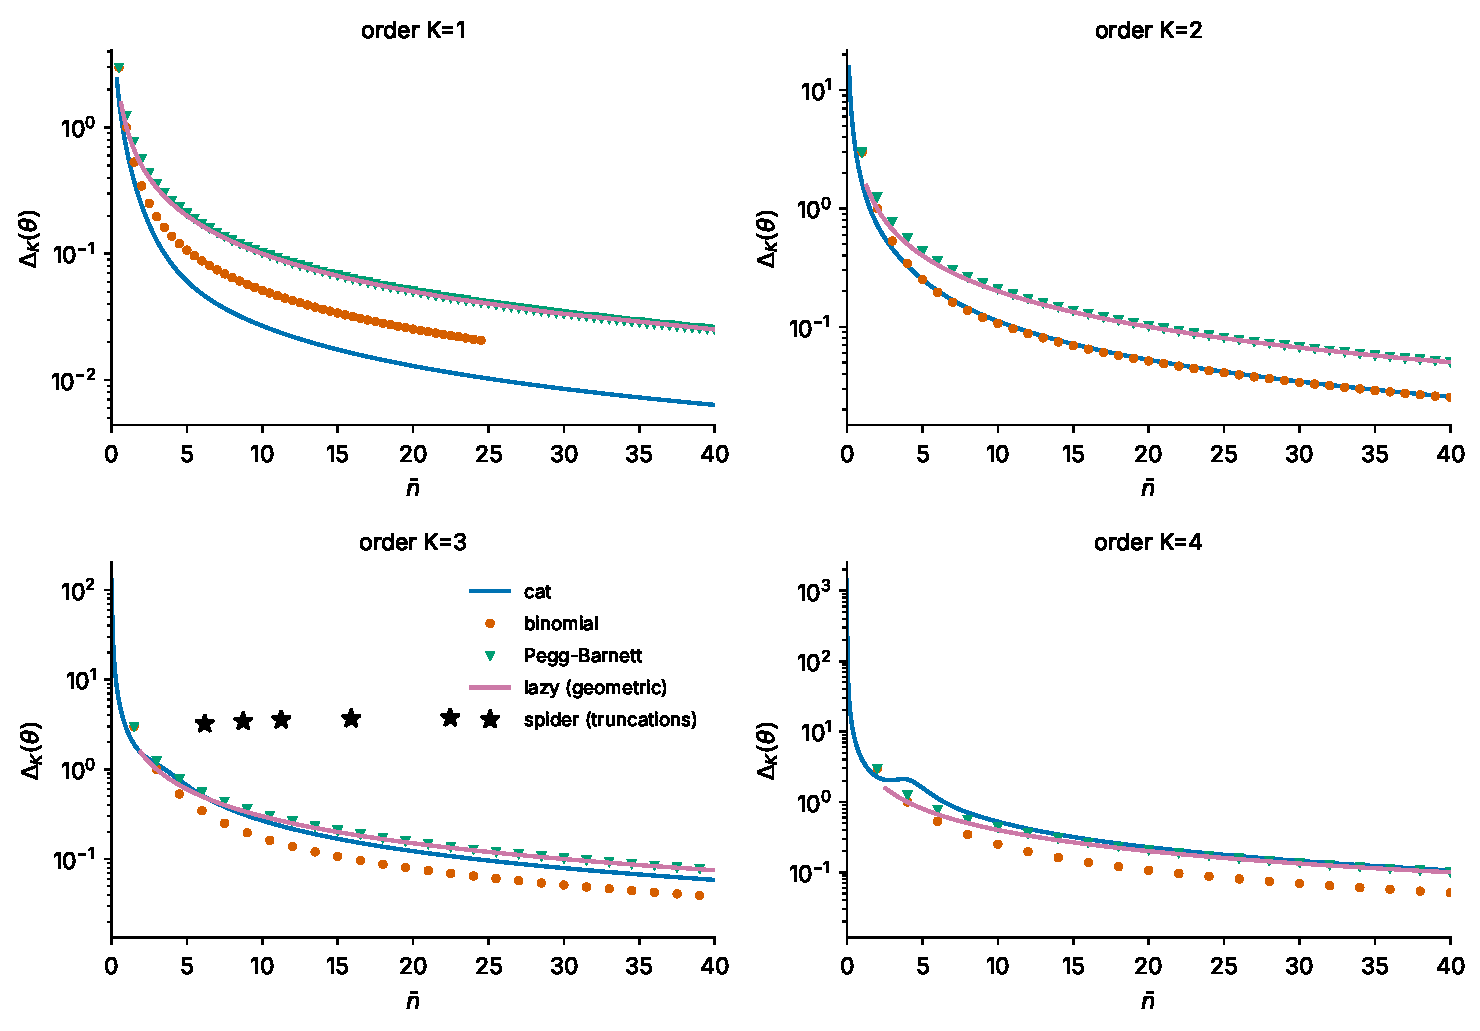
\includegraphics[width=\columnwidth]{embedded_phase_uncertainty_vs_nbar}
  \caption{\label{fig:epu}Embedded phase uncertainty against mean photon number
  for cat, binomial, Pegg--Barnett and geometric (``lazy'') primitives of order
  $K=1$--$4$, and for truncations of the spider state (stars; $K=3$ only, the
  even-$K$ and $K=1$ protocols have no non-trivial optimum).}
\end{figure}

\subsection{What the spider code has that no other code has}
The one genuinely new feature is certification. Cat and binomial codewords are
verified by Wigner tomography. The spider state is by definition the top
eigenvector of an observable, $\hat Q_K$, that is measured by sign
measurements of $x$ at $K$ times---the simplest measurement an oscillator
admits. For any state $\rho$,
$\mathrm{tr}(\rho\hat Q_K)\le q_dF+q_{d-1}(1-F)$ with
$F=\bra{S_K}\rho\ket{S_K}$, hence
\begin{equation}
  F\;\ge\;\frac{\mathrm{tr}(\rho\hat Q_K)-q_{d-1}}{q_d-q_{d-1}}
  =1-\frac{q_d-\mathrm{tr}(\rho\hat Q_K)}{\epsilon}.
  \label{eq:witness}
\end{equation}
A measured score within $0.01$ of the maximum certifies a fidelity of at least
$0.76$ with $\ket{S_3}$, device-independently. (The original manuscript in the
repository sketched this bound in a weaker form.)

% ----------------------------------------------------------------------------
\section{Knill--Laflamme verdict}\label{sec:kl}
% ----------------------------------------------------------------------------
A code corrects the error set $\{\hat E_a\}$ if and only if
\cite{knill1997,nielsenchuang}
\begin{equation}
  \bra{i_L}\hat E_a^\dagger\hat E_b\ket{j_L}=C_{ab}\,\delta_{ij}. \label{eq:kl}
\end{equation}
For $i\ne j$ this is orthogonality: no error maps one codeword onto the other.
For $i=j$ it is non-deformation: both codewords must see the same error
statistics, otherwise the syndrome measurement learns, and therefore destroys,
the logical information. For an RSB code and loss errors $\hat a^l$ with
$l<K$, orthogonality is automatic from the Fock-grid spacing. Non-deformation
for a single loss reads $\bra{0_L}\n\ket{0_L}=\bra{1_L}\n\ket{1_L}$: the two
codewords must have the same mean photon number.

\begin{table}[t]
\caption{\label{tab:kl}Knill--Laflamme matrix elements for order-3 codes with
the error set $\{\hat 1,\hat a,\hat a^2,\n\}$ (truncation 600). ``Orth.'' is
the largest $|\bra{0_L}\hat E_a^\dagger\hat E_b\ket{1_L}|$; the deformation
columns give $\bra{1_L}\hat E^\dagger\hat E\ket{1_L}-\bra{0_L}\hat E^\dagger\hat
E\ket{0_L}$.}
\begin{ruledtabular}
\begin{tabular}{lcccc}
 code & orth. & $\hat a$ & $\hat a^2$ & $\n$\\
\hline
 spider, $K=3$ & $0$ & $15.75$ & $247$ & $262$\\
 cat, $\alpha=2$ & $0$ & $-1.76$ & $-15.9$ & $-17.6$\\
 cat, $\alpha=3$ & $0$ & $0.36$ & $3.43$ & $3.79$\\
 binomial, $L=2$ & $0$ & $0$ & $-9.0$ & $-9.0$\\
 binomial, $L=4$ & $0$ & $0$ & $0$ & $0$\\
\end{tabular}
\end{ruledtabular}
\end{table}

Table~\ref{tab:kl} shows the verdict. The spider code passes orthogonality
exactly and fails non-deformation already for a single loss, by an amount of
order $\bar n$ itself; the relative mismatch
$(\bar n_1-\bar n_0)/(\bar n_1+\bar n_0)$ locks at $0.50$ for every truncation
(Fig.~\ref{fig:repair}, left inset of notebook 03). By contrast the binomial
code with $L=4$ satisfies all conditions exactly, and the cat code
approaches them exponentially in $|\alpha|^2$. The spider code is an
error-\emph{detecting} but not an error-\emph{correcting} code.

\begin{figure*}[t]
  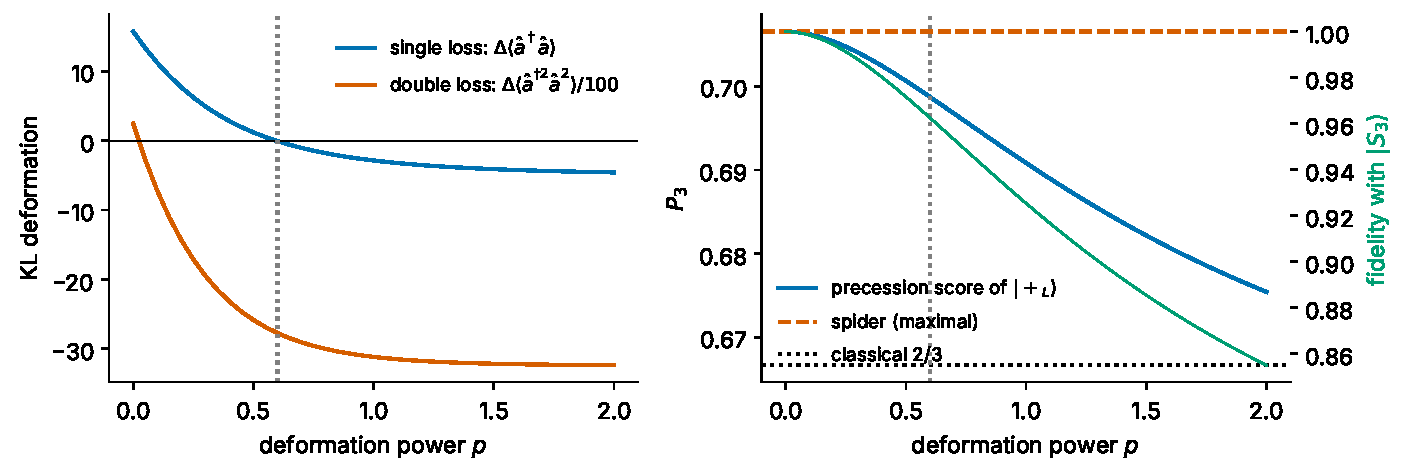
\includegraphics[width=0.95\textwidth]{spider_kl_repair_tradeoff}
  \caption{\label{fig:repair}Attempting to repair the spider code by
  reweighting $\ket{1_L}\to\mathcal N(\n+1)^{-p/2}\ket{1_L}$. Left: the
  Knill--Laflamme deformation for one and two losses as a function of $p$; the
  single-loss deformation vanishes at $p\simeq0.6$ while the double-loss one
  is in the thousands. Right: precession score (blue) and fidelity with
  $\ket{S_3}$ (green) of the resulting $\ket{+_L}$; the repaired state is no
  longer the spider state.}
\end{figure*}

Could the coefficients be ``renormalised'' to repair this? Figure~\ref{fig:repair}
answers with the simplest one-parameter family. One parameter fixes one
condition: at $p\simeq0.6$ the single-loss deformation vanishes, but the
double-loss deformation remains in the thousands, and each further error
would demand a further parameter---the family converges to a binomial-like
amplitude profile, not to the spider. More importantly, the repaired
$\ket{+_L}$ is no longer the top eigenvector of $\hat Q_K$: its score drops
from $0.7066$ to $0.6987$ (still above the classical bound, that part is
robust), so the certificate of Eq.~\eqref{eq:witness} is lost. And no
reweighting of finitely many coefficients touches the infinite energy. Maximal
violation of the precession bound and non-deformation under loss are
incompatible demands on the same set of Fock-grid coefficients.

% ----------------------------------------------------------------------------
\section{The CROT gate from a drive-tuned cross-Kerr interaction}\label{sec:crot}
% ----------------------------------------------------------------------------
\subsection{Why CROT}
If the exotic primitive does not help, the limiting factor of RSB error
correction is not the primitive but the gadgets, which are the same for every
primitive. The hybrid Steane--Knill circuit of Ref.~\cite{grimsmo2020}
(Fig.~\ref{fig:gadget}) couples the data mode (order $K_A$) to an ancilla
(order $K_B$) by
\begin{equation}
  \mathrm{CROT}(\varphi)=e^{i\varphi\n_A\otimes\n_B},\qquad\varphi=\frac{2\pi}{K_AK_B},
\end{equation}
which acts as the identity on the code space and converts a loss of $k$ photons
in the data mode into a rotation by $-2\pi k/(K_AK_B)$ of the ancilla, read
out by a phase measurement. The natural generator of CROT is the cross-Kerr
interaction $\chi_{AB}\n_A\n_B$ between two cavities, which they inherit when
both are dispersively coupled to a common transmon \cite{koch2007,blais2021}.
Zhang \emph{et al.} \cite{zhang2022} showed that an off-resonant drive on the
transmon tunes the inherited self- and cross-Kerr, including through zero.

\begin{figure}[t]
  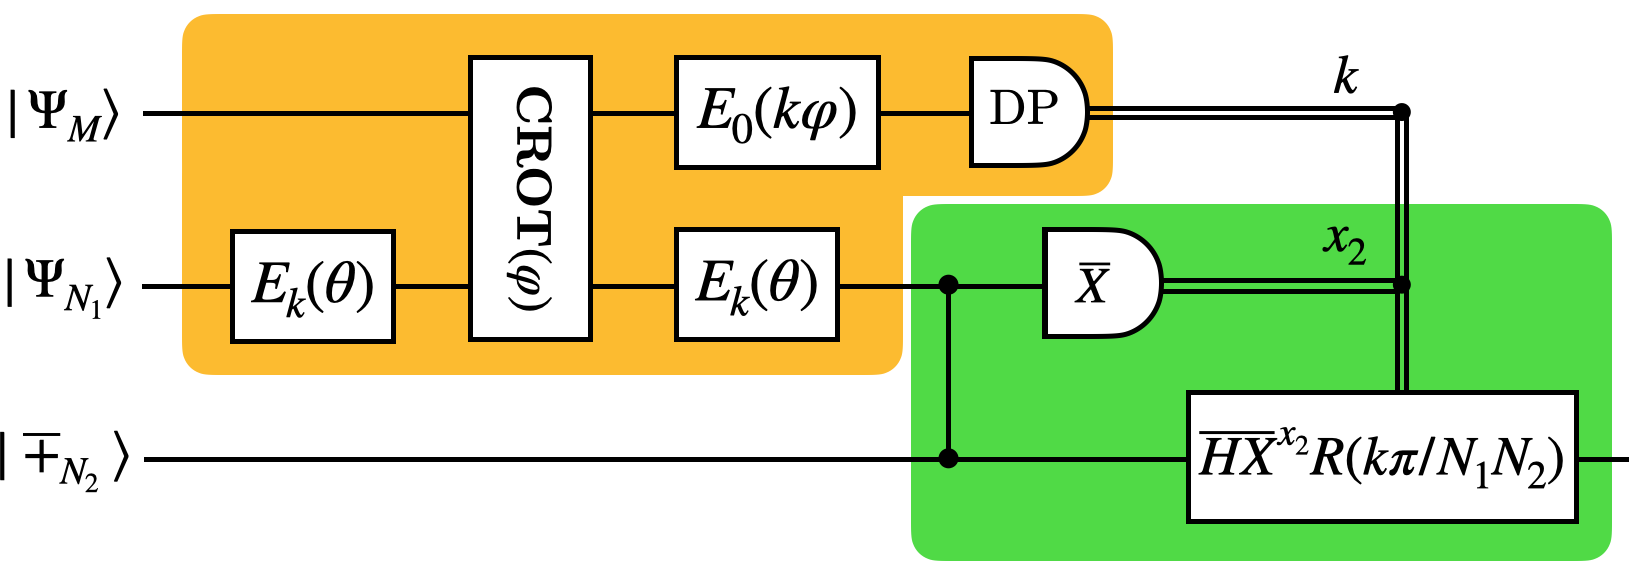
\includegraphics[width=\columnwidth]{steane_knill_gadget}
  \caption{\label{fig:gadget}Hybrid Steane--Knill error-correction gadget for
  rotation codes: a CROT gate between the data mode $\ket{\Psi_{N_1}}$ and an
  ancilla $\ket{\Psi_M}$, a phase measurement (DP) and an $\bar X$ measurement,
  followed by a classically controlled recovery on a fresh mode. Reproduced
  from Grimsmo \emph{et al.}, Phys.\ Rev.\ X \textbf{10}, 011058 (2020),
  CC-BY 4.0.}
\end{figure}

\subsection{Model}
We take a transmon with $\omega_{10}/2\pi=4.936$~GHz and anharmonicity
$\alpha/2\pi=168$~MHz in the Duffing approximation, capacitively coupled to
cavities $A$ and $B$ and driven at $\omega_d$. In the drive frame and after the
rotating-wave approximation \cite{zhang2022},
\begin{align}
  \hat H={}&-\delta_{da}\hat a^\dagger\hat a-\delta_{db}\hat b^\dagger\hat b
  -\delta_{dc}\hat c^\dagger\hat c-\tfrac\alpha2\hat c^\dagger\hat c(\hat c^\dagger\hat c+1)\nonumber\\
  &+\Omega_d(\hat c+\hat c^\dagger)+g_a(\hat a\hat c^\dagger+\mathrm{h.c.})
  +g_b(\hat b\hat c^\dagger+\mathrm{h.c.}),
\end{align}
with $\delta_{dx}=\omega_d-\omega_x$. The dimensionless knobs are
$r_1=\delta_a/\alpha$, $r_2=g_a/\delta_a\ll1$ (dispersive regime),
$r_3=\delta_d/\alpha$ and the drive amplitude $r_4=\Omega_d/\delta_d$. The
cavity nonlinearities are read from the dressed energy ladder $E(N_A,N_B)$ of
the eigenstates adiabatically connected to
$\ket{N_A,N_B}\otimes\ket{\text{transmon ground}}$, obtained by exact
diagonalisation and maximum-overlap labelling:
\begin{align}
  E(N)&=E_0+\delta N+\tfrac K2N^2+\tfrac\beta6N^3+\dots,\\
  \chi_{AB}&=E(1,1)-E(1,0)-E(0,1)+E(0,0).
\end{align}
This dressed-ladder method reproduces the time-domain ``pseudo-experimental''
extraction of the original notebooks (fitting Wigner-function evolutions) a
thousand times faster and converges to four digits at modest truncations.

\subsection{Results}
For the baseline $r_1=9.64$, $r_2=0.064$, $r_3=0.08$ and no drive, the
inherited self-Kerr is $K_A=-2.62$~kHz. Under the drive it changes sign,
passing through a Kerr-free point near $|\Omega_d/\delta_d|^2\simeq0.05$, and
reaches $+14$~kHz (Fig.~\ref{fig:kerr}, left), in agreement with
Ref.~\cite{zhang2022}. With a second cavity on the other side of the transmon
($r_{1b}=-9$, $r_{2b}=0.05$, $r_3=0.26$) the cross-Kerr grows from
$-1.40$~kHz to $+5.75$~kHz, a four-fold enhancement in magnitude
(Fig.~\ref{fig:kerr}, right). But $K_A$, $K_B$ and $\chi_{AB}$ all cross zero
at nearby yet different drive amplitudes, and everywhere
$|K_A|,|K_B|\sim|\chi_{AB}|$: one transmon with one drive can null one
self-Kerr, not both, and not at the maximum of $\chi_{AB}$.

\begin{figure*}[t]
  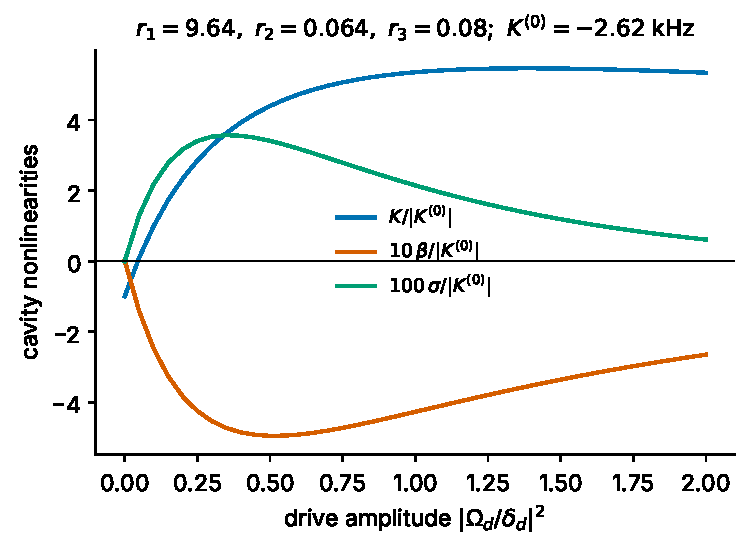
\includegraphics[width=0.48\textwidth]{self_kerr_vs_drive_one_cavity}\hfill
  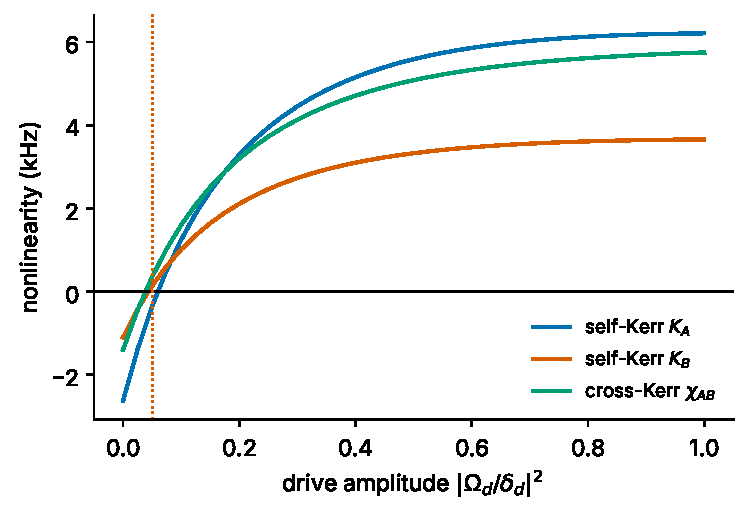
\includegraphics[width=0.48\textwidth]{cross_kerr_vs_drive_two_cavities}
  \caption{\label{fig:kerr}Left: drive-induced nonlinearities of one cavity,
  normalised to the undriven $|K^{(0)}|$, in the format of
  Ref.~\cite{zhang2022}. Right: self-Kerr $K_A$, $K_B$ and cross-Kerr
  $\chi_{AB}$ of two cavities sharing a driven transmon; dotted lines mark the
  Kerr-free points.}
\end{figure*}

The consequence for the gate is severe. We target $\varphi=2\pi/9$ between an
order-3 binomial data code ($L=4$, the Knill--Laflamme-correct code of
Table~\ref{tab:kl}) and an order-3 cat ancilla, generated by
$\hat H_{\rm eff}=\chi_{AB}\n_A\n_B+\tfrac{K_A}2\n_A^2+\tfrac{K_B}2\n_B^2$ for
$t_g=|\varphi|/(2\pi|\chi_{AB}|)$, and compute the average gate fidelity with
the ideal CROT on the logical two-qubit subspace (leakage counted as error).
At the strongest drive $t_g=19\,\mu$s, short compared with millisecond cavity
lifetimes. Without self-Kerr the fidelity is unity to numerical precision,
since $\n_A\n_B$ is the exact generator; with the simulated self-Kerr it lies
between $0.07$ and $0.43$ over the whole drive range (Fig.~\ref{fig:crot},
left), because a 5~kHz self-Kerr accumulates phases of order $\pi\bar n^2$
during the gate. A $99\%$ CROT tolerates a residual self-Kerr of only
$|K|\lesssim7\times10^{-3}|\chi_{AB}|$, about $40$~Hz for
$\chi_{AB}=5.8$~kHz (Fig.~\ref{fig:crot}, right).

\begin{figure*}[t]
  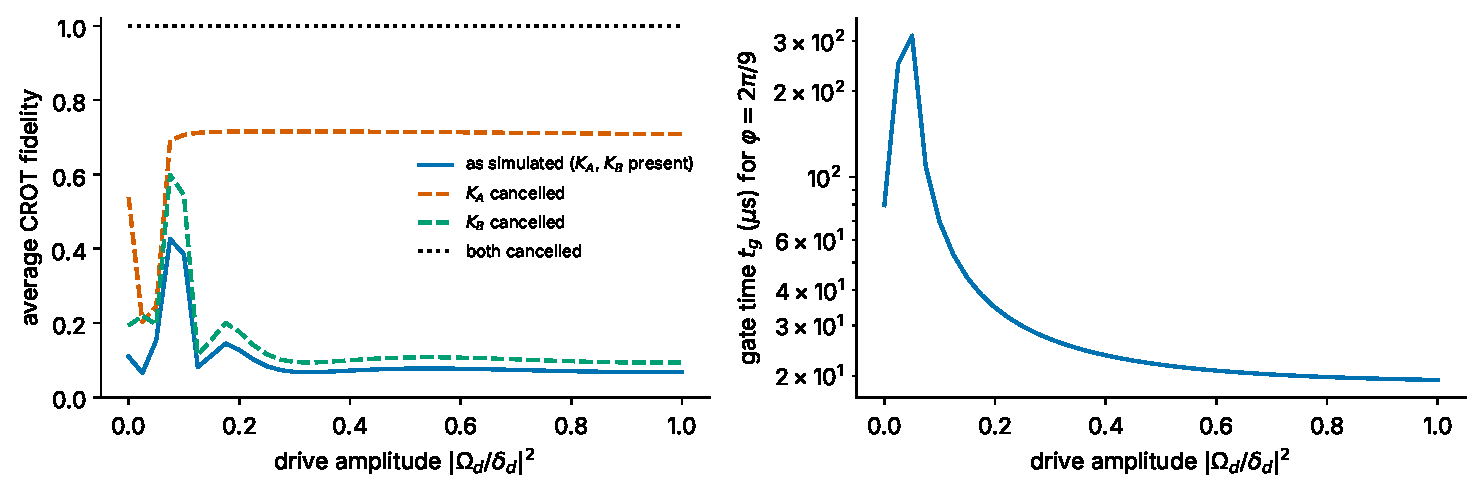
\includegraphics[width=0.62\textwidth]{crot_fidelity_and_time_vs_drive}\hfill
  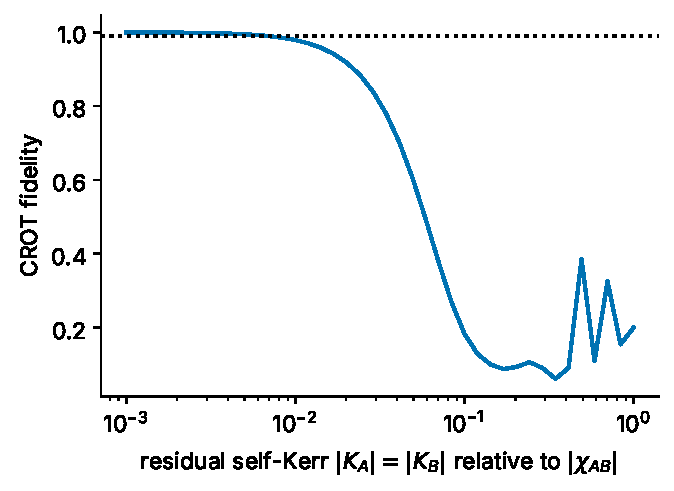
\includegraphics[width=0.34\textwidth]{crot_fidelity_vs_residual_self_kerr}
  \caption{\label{fig:crot}Left: average fidelity of the cross-Kerr CROT
  ($\varphi=2\pi/9$) as simulated and with one or both self-Kerrs cancelled,
  and the gate time, against the drive amplitude. Right: fidelity against the
  residual self-Kerr relative to the cross-Kerr; the dotted line is $0.99$.}
\end{figure*}

The original project explored one way out: a four-mode chain
$A$--$q_c$--$B$--$q_b$ with a second transmon and a second drive, so that the
drive on $q_c$ enhances $\chi_{AB}$ while the drive on $q_b$ nulls $K_B$. The
recovered data (Fig.~\ref{fig:legacy}) show such an operating point, with
$\chi_{AB}\simeq48$~kHz, $K_B=0$, and a residual $K_A\simeq-12$~kHz. This
is the side-transmon cancellation that the published scheme adopts.

\subsection{The targeted resonance of Qin \emph{et al.}}
The project was completed after the above study by Qin, My, Copetudo,
Kasper, Gao and Ng \cite{qin2026}, whose resolution is not to drive harder
but to drive at the right place. In the frame of a single-tone drive the
dressed transmon can convert an $a$ photon into a $b$ photon plus one
transmon excitation when $D^{\rm res}=\omega_a-(\omega_b+\epsilon_{10})\approx0$.
Near this resonance the cross-Kerr, which involves both cavities, is
enhanced as $1/D^{\rm res}$, whereas the self-Kerrs, which involve one cavity,
are not; the residual self-Kerr of cavity $a$ is then cancelled by a driven
\emph{side} transmon coupled only to $a$, the scheme already present in the
four-mode chain of Fig.~\ref{fig:legacy}. Their parameters are
$\omega_a/2\pi=4.0$, $\omega_b/2\pi=4.3$, $\omega_{10}/2\pi=4.65$~GHz,
$\alpha/2\pi=0.2$~GHz, $|g_a/\delta_a|=0.04$, $|g_b/\delta_b|=0.03$ and
$|\Omega_d/\delta_d|=1$, with the drive detuning $\delta_d/\alpha$ brought
up to $0.835$, just below the resonance at $\simeq0.88$.

Feeding these parameters to the dressed-ladder code reproduces the picture
without any perturbation theory (Fig.~\ref{fig:qin}). Approaching the
resonance from below, $|\chi_{AB}|$ grows from $0.7$~kHz to $37$~kHz at the
working point (on-off ratio $\simeq52$; the perturbative estimate of
Ref.~\cite{qin2026} is $>60$) and to $60$~kHz just before the hybridisation
window, while $K_B$ decreases towards zero and $K_A$ stays at a few kHz, so
that $|\chi_{AB}/K_A|\simeq4$--$9$ instead of the $\simeq1$ of the untargeted
sweep. Inside the window $0.86\lesssim\delta_d/\alpha\lesssim0.91$ the dressed
state $\ket{1,0,0}$ hybridises with $\ket{0,1,1}$ and the ladder is no longer
defined; on the far flank, $\delta_d/\alpha\simeq0.92$, the numerics even show
$K_A$ crossing zero with $\chi_{AB}\simeq48$~kHz. For their
error-correction example---an order-2 binomial data code, an order-1 cat
ancilla and a first CROT angle $\varphi=2\pi/(NM)=\pi$, gate time
$14\,\mu$s at the working point---the two-mode average gate fidelity of our
diagonal model is $0.43$ with the central transmon alone and $0.69$ once the
side transmon cancels $K_A$; but the remaining error is then a Kerr phase on
the ancilla alone, which commutes with CROT and leaves the reduced state of
the data mode untouched. The \emph{data-rail} fidelity, which is the figure
reported in Ref.~\cite{qin2026}, is $0.978$ without and $1.000$ with the side
transmon in our model, consistent with their $0.96$--$0.99$ (limited by
higher-order and state-dependent Kerr terms that a diagonal model omits).
With these gates they simulate the full Grimsmo gadget and obtain an
error-correction cycle of $\sim19\,\mu$s that beats the bare cavity at high
loss rates, at a cost of $7$--$12\%$ relative to ideal CROTs.

\begin{figure*}[t]
  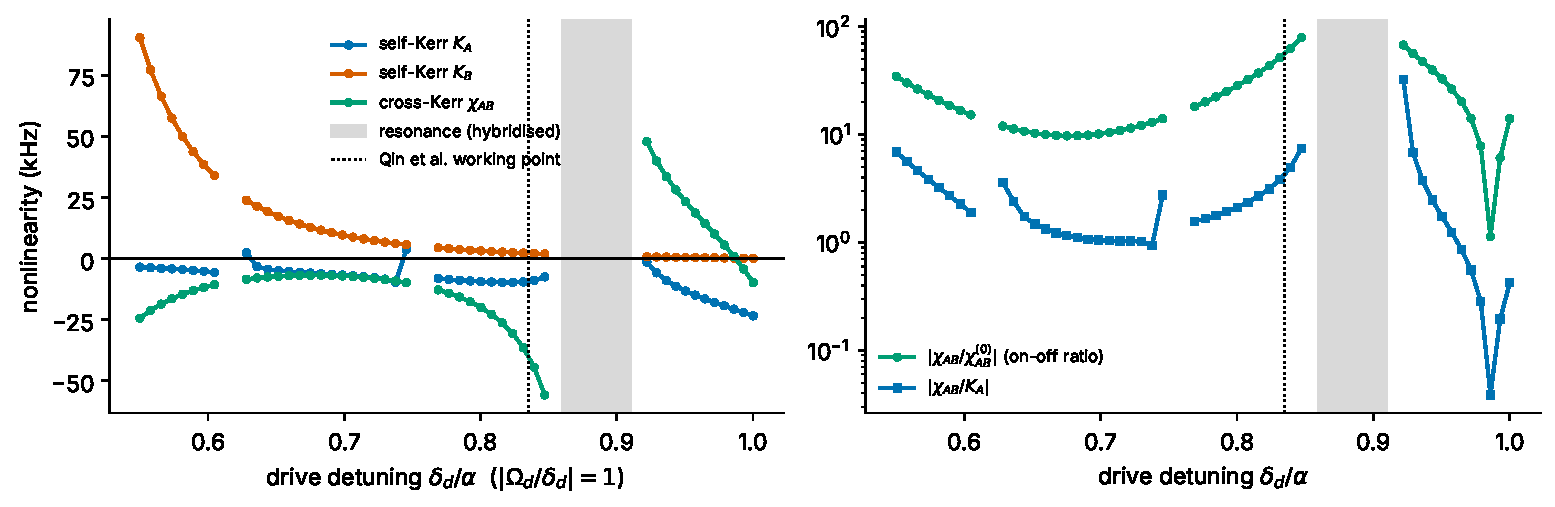
\includegraphics[width=0.95\textwidth]{qin2026_targeted_resonance_cross_kerr}
  \caption{\label{fig:qin}Dressed-ladder reproduction of the targeted
  resonance of Qin \emph{et al.} \cite{qin2026}. Left: $K_A$, $K_B$ and
  $\chi_{AB}$ against the drive detuning at $|\Omega_d/\delta_d|=1$; the shaded
  window is the hybridised region where the ladder is undefined, the dotted
  line their working point. Right: on-off ratio of the cross-Kerr and the
  ratio $|\chi_{AB}/K_A|$.}
\end{figure*}

\begin{figure*}[t]
  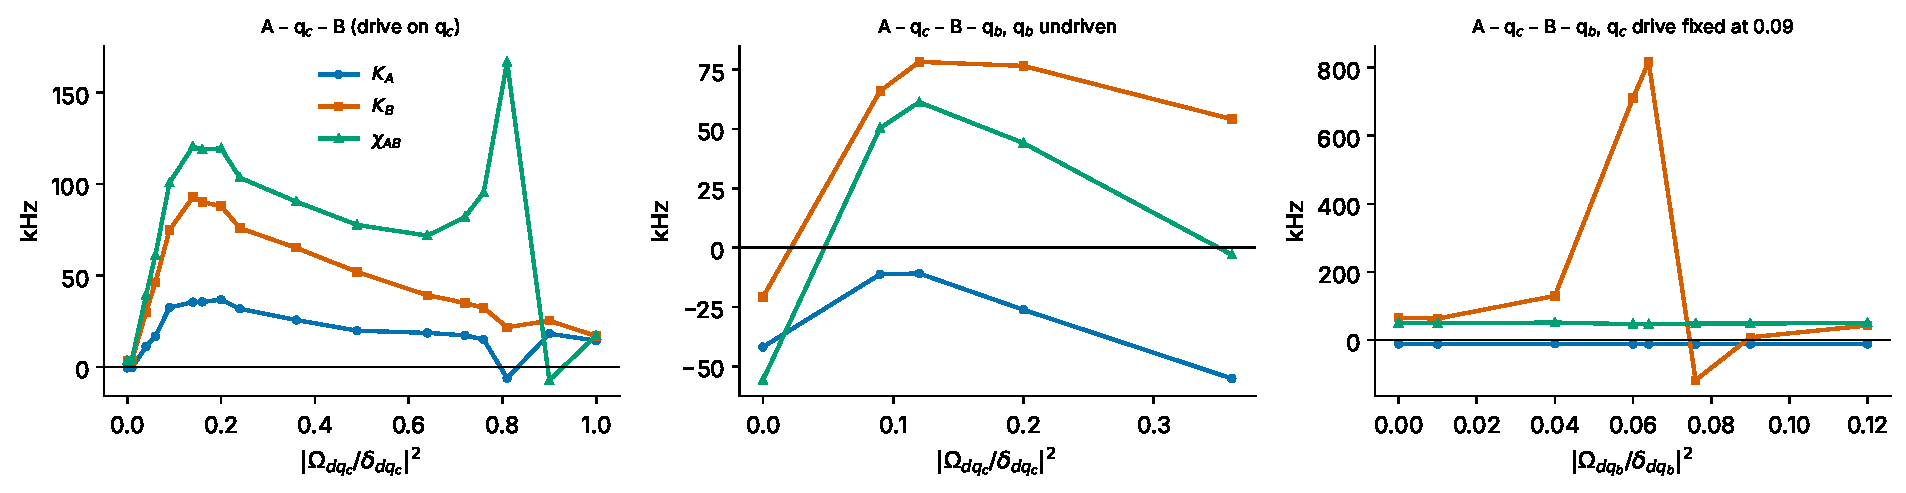
\includegraphics[width=0.95\textwidth]{legacy_four_mode_kerr_chain}
  \caption{\label{fig:legacy}Nonlinearities of the chains $A$--$q_c$--$B$
  (left) and $A$--$q_c$--$B$--$q_b$ (middle, right) recovered from the
  original project ($\alpha/2\pi=125$~MHz, larger couplings than in
  Fig.~\ref{fig:kerr}). In the right panel the $q_c$ drive is fixed at
  $|\Omega/\delta|^2=0.09$ and the $q_b$ drive is swept; $K_B$ crosses zero
  near $0.074$ while $\chi_{AB}$ stays near $50$~kHz.}
\end{figure*}

% ----------------------------------------------------------------------------
\section{Conclusion and outlook}\label{sec:outlook}
% ----------------------------------------------------------------------------
We followed a state from a test of quantumness to a bosonic code and back to
the hardware. The spider state of Zaw \emph{et al.} is a legitimate order-$K$
rotation-symmetric primitive, and the only one whose preparation can be
certified by sign measurements alone, through the spectral-gap witness of
Eq.~\eqref{eq:witness}. As a code it detects $K-1$ losses but does not correct
them: its two codewords carry mean photon numbers in a fixed ratio of three,
the Knill--Laflamme non-deformation condition fails by an amount of order
$\bar n$, and any reweighting that repairs one condition abandons the maximal
violation that defines the state while leaving its infinite energy intact.
The spider is a witness, not a code.

The obstacle to rotation-code error correction is therefore in the gadgets,
and we quantified the central one. An untargeted drive-tuned cross-Kerr
interaction between two cavities gives a CROT gate in tens of microseconds,
but the same mechanism produces self-Kerr of comparable size, and the gate
tolerates only a residual of order $10^{-2}$ of the cross-Kerr. The published
completion of the project \cite{qin2026} resolves this by placing a single-tone
drive next to the $a\leftrightarrow b$ conversion resonance, which enhances the
cross-Kerr by nearly two orders of magnitude while leaving the self-Kerrs
small, and by cancelling the residual with a driven side transmon---the very
chain explored in the recovered four-mode data. Our dressed-ladder numerics
reproduce the resonance, the on-off ratio and the data-rail fidelity of that
scheme.

Three directions follow. (i)~\emph{Beyond the diagonal model}: the
$0.96$--$0.99$ gate fidelities of Ref.~\cite{qin2026} are limited by
higher-order and state-dependent Kerr terms; a selective number-dependent
phase (SNAP) correction or a Kerr echo could remove what the side transmon
leaves. (ii)~\emph{Phase measurement}: the second half of the gadget needs a canonical phase
measurement on the ancilla; the adaptive feedback scheme of Martin
\emph{et al.} \cite{martin2020} is the natural candidate, and the embedded
phase uncertainty of Fig.~\ref{fig:epu} ranks the ancilla primitives for it.
(iii)~\emph{Precession witness as a diagnostic}: although the spider code
fails, the precession score is a cheap, device-independent non-classicality
witness for \emph{any} rotation-symmetric state, since $\hat Q_K$ is block
diagonal in exactly the symmetry sectors the codes live in; using it to
monitor cat- and binomial-code preparation seems the most useful legacy of the
spider.

All numerics are reproducible from the accompanying repository, which contains
the Python modules, the four notebooks that carry the argument of this paper,
and the recovered data and notes of the original project.

\begin{acknowledgments}
The author thanks the Centre for Quantum Technologies for hospitality during
the original project. The first leg of the project was conducted in the group of Valerio Scarani. The second leg was in the group of Hui Khoon Ng. Results were obtained during the project timeline (2023-2024). LLMs were used to summarize, organize, and write up this report. The numerical work uses NumPy, SciPy and QuTiP.
\end{acknowledgments}

\appendix
% ----------------------------------------------------------------------------
\section{Matrix elements of the half-line projector}\label{app:pos}
% ----------------------------------------------------------------------------
With $\psi_n$ the oscillator eigenfunctions, $-\tfrac12\psi_n''+\tfrac12x^2\psi_n=(n+\tfrac12)\psi_n$.
Multiplying the equations for $m$ and $n$ by $\psi_n$ and $\psi_m$, subtracting and
integrating over $x>0$ gives
$(m-n)\int_0^\infty\psi_m\psi_n\,dx=\tfrac12\left[\psi_n\psi_m'-\psi_m\psi_n'\right]_{x=0}$,
which is the closed form used in the text. The boundary values are
$\psi_{2j}(0)=\pi^{-1/4}(-1)^j\sqrt{(2j)!}/(2^jj!)$, $\psi_{2j+1}(0)=0$, and
$\psi_n'(0)=[\sqrt n\,\psi_{n-1}(0)-\sqrt{n+1}\,\psi_{n+1}(0)]/\sqrt2$, evaluated in log
space for large $n$. The diagonal elements are $1/2$ by parity.

% ----------------------------------------------------------------------------
\section{Numerical details}\label{app:num}
% ----------------------------------------------------------------------------
The spider state is the top eigenvector of the residue-0 block of $\hat Q_K$,
of dimension $n$ for a Fock cutoff $Kn$; dense diagonalisation up to $n=7000$
takes under a minute. The Knill--Laflamme tensor is evaluated at a cutoff of
600 with the errors $\{\hat1,\hat a,\hat a^2,\n\}$. Cavity--transmon ladders
use QuTiP operators with truncations (20, 8) for one cavity and (8, 8, 6) for
two cavities; the smallest overlap between a coupled eigenstate and its bare
label is $0.90$ (one cavity) and $0.97$ (two cavities). The CROT fidelity is
$F=(|\mathrm{tr}M|^2+\mathrm{tr}M^\dagger M)/[d(d+1)]$ with $d=4$ and
$M=B^\dagger U_{\rm ideal}^\dagger U B$, $B$ the orthonormal logical basis.

\bibliographystyle{\ifnum\revtexfallback=1 unsrtnat\else apsrev4-2\fi}
\bibliography{references}

\end{document}
